% 原作者:https://jevon.org/wiki/Fancy_Quotation_Boxes_in_Latex(这个框框的形式是我在此基础上改的)
\documentclass{book}
\usepackage{newtxtext}
\usepackage[marginparwidth={4cm},lmargin={1cm}, rmargin={5cm}]{geometry}
\usepackage[dvipsnames,svgnames,x11names]{xcolor}
\usepackage[strict]{changepage} % 提供一个 adjustwidth 环境
\usepackage{framed} % 框包
\usepackage{xeCJK}%中文包
\usepackage{amsmath}%写连等式对齐包
\usepackage{graphicx}%插入图片
\usepackage{wallpaper}%插入背景图
\usepackage{indentfirst}%latex第一段首行不缩进,看着不爽,于是用包使每段都不缩进
%\usepackage{titlesec}如有需要设置各级标题
%\usepackage{ctex}如有需要设置中文字体
\usepackage{graphicx}%图片

\geometry{a4paper,centering,scale=0.8}
\definecolor{formalshade}{rgb}{0.95,0.95,1} % 文本框颜色
% ------------------******-------------------
% 注意行末需要把空格注释掉,不然画出来的方框会有空白竖线
\definecolor{greenshade}{rgb}{0.92,1,0.92}
\definecolor{grayshade}{rgb}{0.90,0.90,0.90}
%蓝紫框--------------------------------------------
\newenvironment{formal1}{%
\def\FrameCommand{%
\hspace{1pt}%
{\color{DarkBlue}\vrule width 2pt}%
{\color{SteelBlue}\vrule width 4pt}%
\colorbox{formalshade}%
}%
\MakeFramed{\advance\hsize-\width\FrameRestore}%
\noindent\hspace{-4.55pt}% disable indenting first paragraph
\begin{adjustwidth}{}{7pt}%
\vspace{2pt}\vspace{2pt}%
}
{%
\vspace{2pt}\end{adjustwidth}\endMakeFramed%
}
%绿框---------------------------------------
\newenvironment{formal2}{%
\def\FrameCommand{%
\hspace{1pt}%
{\color{Green}\vrule width 2pt}%
{\color{DarkSeaGreen1}\vrule width 4pt}%
\colorbox{greenshade}%
}%
\MakeFramed{\advance\hsize-\width\FrameRestore}%
\noindent\hspace{-4.55pt}% disable indenting first paragraph
\begin{adjustwidth}{}{7pt}%
\vspace{2pt}\vspace{2pt}%
}
{%
\vspace{2pt}\end{adjustwidth}\endMakeFramed%
}
%灰框---------------------------------------
\newenvironment{formal3}{%
\def\FrameCommand{%
\hspace{1pt}%
{\color{darkgray}\vrule width 2pt}%
{\color{Ivory4}\vrule width 4pt}%
\colorbox{grayshade}%
}%
\MakeFramed{\advance\hsize-\width\FrameRestore}%
\noindent\hspace{-4.55pt}% disable indenting first paragraph
\begin{adjustwidth}{}{7pt}%
\vspace{2pt}\vspace{2pt}%
}
{%
\vspace{2pt}\end{adjustwidth}\endMakeFramed%
}
%天蓝框---------------------------------------
\newenvironment{formal4}{%
\def\FrameCommand{%
\hspace{1pt}%
{\color{SkyBlue}\vrule width 2pt}%
{\color{Cyan1}\vrule width 4pt}%
\colorbox{LightCyan1}%
}%
\MakeFramed{\advance\hsize-\width\FrameRestore}%
\noindent\hspace{-4.55pt}% disable indenting first paragraph
\begin{adjustwidth}{}{7pt}%
\vspace{2pt}\vspace{2pt}%
}
{%
\vspace{2pt}\end{adjustwidth}\endMakeFramed%
}
%粉框---------------------------------------
\newenvironment{formal5}{%
\def\FrameCommand{%
\hspace{1pt}%
{\color{HotPink}\vrule width 2pt}%
{\color{LightPink}\vrule width 4pt}%
\colorbox{MistyRose}%
}%
\MakeFramed{\advance\hsize-\width\FrameRestore}%
\noindent\hspace{-4.55pt}% disable indenting first paragraph
\begin{adjustwidth}{}{7pt}%
\vspace{2pt}\vspace{2pt}%
}
{%
\vspace{2pt}\end{adjustwidth}\endMakeFramed%
}
%首段首行缩进--------------------------------------
\setlength{\parindent}{0em}

% ------------------******-------------------
% ------------------******-------------------
% ------------------******-------------------
% ------------------******------------------
\begin{document}
 \begin{titlepage}
 \newgeometry{left=3cm,right=3cm}
 \ThisCenterWallPaper{1.255}{fig/8.jpg}
 \color{darkgray} 
 \begingroup
 \thispagestyle{empty}
 \centering
 \vspace*{5cm}
 \par\normalfont\fontsize{35}{35}\sffamily\selectfont
 \textbf{C/C++}\\ 
 {\LARGE 002 Intro}\par % Book title
 \vspace*{1cm}
 {\Huge Notes of Practice}\par % Author name
 \endgroup
 \end{titlepage}



 \section{Introduction to Computers, the Internet and the Web}
\marginpar{下载Mingw-w64要挂梯子\\
没有梯子就在网上找网盘\\
\\
将文件下载到没有中文和空格的路径(重点)\\
\\
电脑path选账户环境变量,防止系统崩掉\\
\\
vscode配置的有点多,下方安利一个程序\\
}


\par \begin{enumerate}
 \item 下载Mingw-w64(就是它的版本问题,不要点大download,即10.0.0版,在file里找一个8.10.0版本即可)
 \item 下载7z(官网上下载的需要解压)
 \item 添加环境变量path
 \item 检验配置
 \item 下载vscode插件
 \item 配置vscode
\end{enumerate}

\color{darkgray}
 \definecolor{shadecolor}{rgb}{0.90,0.9,0.90}
 \begin{shaded}
 {\subsection[short]{Computing}}
\end{shaded}
\color{black}

\begin{formal4}
以下分别是mingw-w64和7z的官网\\    
\begin{itemize}
\item https://sourceforge.net/projects/mingw-w64/files/
\item https://www.7-zip.org/download.html\\
\end{itemize}
再给大家安利一个程序,可以帮你配置好vscode,一次没配好还可以删了重配\\
一开始是自己慢慢敲的,结果要反复调,用了这个就很省事。\\
VS Code Config Helper,链接https://v4.vscch.tk/,免费真香。
\end{formal4}

\color{darkgray}
 \definecolor{shadecolor}{rgb}{0.90,0.9,0.90}
 \begin{shaded}
 {\subsection[short]{Number System}}
\end{shaded}
\color{black}
\begin{itemize}
    \item Binary System
    Used in electronic devices (computers) as a
    series of "off" and "on" switches.\\
    A way to write numbers using only two digits
    (‘bits’): 0 and 1 (base2).\\
    Each digit's place value is twice as much as
    that of the next digit to the right and the place
    value increases by a power of two (1's, 2's,
    4's place, etc.).\\
    In decimal, each digit holds ten values, and
    the place value increases by a power of ten
    (1's, 10's, 100's place, etc.).\\
    \item hexadecimal System\\
    hexadecimal (also base16, or hex) is a positional numeral
    system with a radix, or base, of 16.\\
    It uses sixteen distinct symbols, most often
    the symbols 0–9 to represent values zero to
    nine, and A, B, C, D, E, F (or alternatively a–f)
    to represent values ten to fifteen.
\end{itemize}
\begin{formal2}
\begin{itemize}
\item  Decimal Conversion
\end{itemize}
在mingw64里找到文件夹“bin”,复制路径\\
在windows里搜索“账户环境变量”点进去,找到Path,打开在下面加一行,把复制的路径粘贴进去\\
如果系统不一样,是写一排的,就打英文分号补后面\\
\begin{itemize}
\item Hex-Binary Convertion
\end{itemize}
打开cmd,输入“where gcc”后弹出路径\\
输入“gcc --version”后弹出gcc版本信息
\end{formal2}

\color{darkgray}
 \definecolor{shadecolor}{rgb}{0.90,0.9,0.90}
 \begin{shaded}
 {\subsection[short]{Modern Computer}}
\end{shaded}
\color{black}
Computers are good at representing/manipulating
numbers. We need to tell the computer exactly what to do
Sequence of instructions is called a computer
program

\begin{figure}[!h]
    \centering
    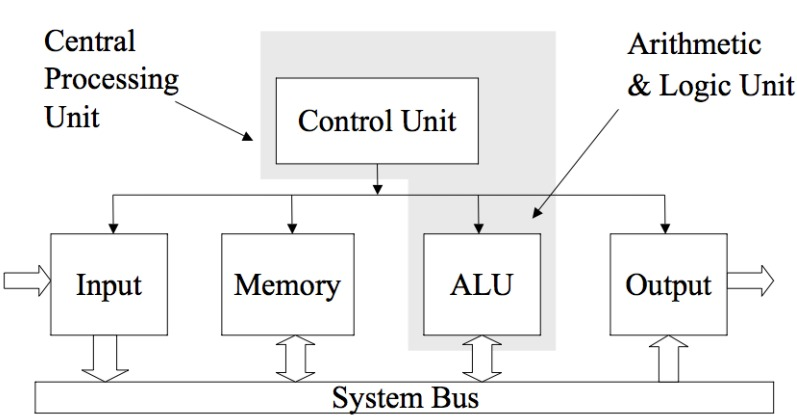
\includegraphics[scale=0.3]{fig/9.jpeg}
    \caption{Architecture of the Modern Computer}
\end{figure} 
\begin{formal1}
\begin{itemize}
\item ALU or Arithmetic and Logic Unit (算术逻
辑 单 元 ) processes data (adding, AND,
etc.)\\
Ø Facilitates decisions by comparing
numbers.\\
Ø Check overflow.
\item Control Unit (控制单元) controls other
units by turning on access to them as
needed.
\item The Control Unit and ALU are the heart
of the Central Processing Unit (CPU - 中
央处理器).\\
The CPU has a special ‘memory’ called
registers and can:
\begin{enumerate}
    \item Fetch instructions from the main memory.
    \item Execute them and hold results in registers.
    \item Pass and store results in memory,and
    \item (based on results) branch to different
\end{enumerate}
\item A computer memory (计算机内存) is an
electronic holding place stores
information.\\
\marginpar{Ø Primary memory:
Ø Read-Only Memory (ROM) – Stores
important information to operate the
system.
Ø It is non-volatile (can not be erased)
}
\end{itemize}
\end{formal1}

\section{网络教程}
\marginpar{多看看官网总是好的\\
}
\begin{itemize}
    \item https://zhuanlan.zhihu.com/p/77074009(小白教程)
    \item https://code.visualstudio.com/docs/cpp/config-mingw(官方教程很详细,但是实操起来缺少点细节)
    \item https://code.visualstudio.com/docs/cpp/cpp-debug(官方debug教程)
\end{itemize}

\section{关于Dev-C++}
为什么我在有这么方便统一的软件情况下还是选择配置vscode。
\begin{itemize}
    \item 首先,我是颜狗lol
    \item 不止会用C,我还要用其他语言,把各种语言放在一起写很方便
    \item 学习新技能
    \item vscode yyds
\end{itemize}
但还是要学习dev的,毕竟不是每个环境、每个考场都有vs
\begin{formal2}
最后,既然开了个头,那就把我以后的C语言笔记都放在里面吧
\end{formal2}

\end{document}